\documentclass[pdftex,12pt,a4paper]{article}

\usepackage{float}
\usepackage{graphicx}  
\usepackage[margin=2cm]{geometry}
\usepackage{breakcites}
\usepackage{indentfirst}
\usepackage{pgfgantt}
\usepackage{pdflscape}
\usepackage{float}
\usepackage{epsfig}
\usepackage{epstopdf}
\usepackage[cmex10]{amsmath}
\usepackage{stfloats}
\usepackage{multirow}
\usepackage[%
    pdfborder={0 0 0}
]{hyperref}
\usepackage{listings}
\lstset{frame=tb,
  language=C,
  aboveskip=3mm,
  belowskip=3mm,
  showstringspaces=false,
  columns=flexible,
  basicstyle={\small\ttfamily},
  numbers=none,
  breaklines=true,
  breakatwhitespace=true,
  tabsize=3
}


\title{BLG 312E Homework 3 Report}
\author{Mohamad Chahadeh - 150220901}
\date{30 - 05 - 2023}

\begin{document}

{\def\null\vskip 2em{}\maketitle}

\section{Introduction}
In this Homework, We implemented Bankers' Algorithm, which is a resource allocation and deadlock avoidance algorithm used in operating systems. It is designed to prevent deadlocks by determining whether a particular resource allocation request from processes can be granted safely without causing deadlock.
\subsection{Program Workflow}
\noindent Three input files are given:
\begin{itemize}
    \item \textbf{resources.txt}: contains the \textbf{total} number of resources available in the system for each resource.
    \item \textbf{allocations.txt}: contains the resources \textbf{already allocated} to each process
    \item \textbf{requests.txt}: a.k.a \textbf{needs} table, contains the \textbf{extra resources required} by each process in order for it to \textbf{finish execution}.
\end{itemize}
\textbf{At the start of the program} we are supposed to \textbf{read all three files}, and import the data into array variables, after that, the \textbf{Max table}, which is a table containing the maximum resources needed for process to finish executing, is calculated along the \textbf{available table}, which is a table containing the available resources for use in the system. \\ 
\textbf{After that}, \textbf{the bankers' algorithm is ran} on the arrays to determine if there is a deadlock or not, if there is, the processes causing the \textbf{deadlock are identified} and outputed into the console.

\subsection{The Bankers' Algorithm} \label{algorithm}
The following steps are taken in order:
\begin{enumerate}
    \item the following tables need to be either available or calculated from available data: 
    \begin{enumerate}
        \item Needs (Requests) table: Max - Allocated
        \item Available Resources table: Max Resources - sum(Allocated)
    \end{enumerate}
    \item set $P = 0$
    \item if $P < Num\ of\ Processes$: \textbf{Increment P}, Else: Jump to step 6.
    \item \textbf{if $Needs[Process\ P] \leq Available\ Resources$ }, Then:
    \begin{enumerate}
        \item execute P
        \item Mark P as finished
        \item $Available\ Resource = Needs[Process P] + Available\ Resources$
        \item Jump to step 3.
    \end{enumerate}
    \item  \textbf{else:} Jump to step 3.
    \item \textbf{if all processes finished}, Then there are \textbf{no deadlocks}.
    \item \textbf{if not all processes finished}, Then:
    \begin{enumerate}
        \item if no processes finished in the previous cycle, \textbf{Then there is Deadlock with the unfinished processes}.
        \item if some processes finished in previous cycle, \textbf{Jump to Step 2.}
    \end{enumerate}
\end{enumerate}

\section{Implementation}
\subsection{File reading}
The files' contents were read using the $fopen()$ and $fscanf()$ functions, in the case of the resources file, one for loop was used to append the data to the array, while for the other files, nested for loops were used because they are 2-D array files.

\subsection{Algorithm}
The Algorithm was implemented based on the steps mentioned in the \hyperref[algorithm]{\textbf{Algorithm section} in the introduction} in C language as follows:
\begin{lstlisting}
    int work[MAX_RESOURCE];
    for (int i = 0; i < MAX_RESOURCE; i++) {
        work[i] = available[i];
    }

    int seq_counter = 0;
    while(true) {
        bool found_process = false;

        for (int i = 0; i < MAX_PROCESS; i++) {

            if (finish[i]) continue;
            bool can_execute = true;

            for(int j = 0; j< MAX_RESOURCE; j++) {
                if (need[i][j] > work[j]) {
                    can_execute = false;
                    break;
                }
            }

            if(can_execute) {

                for(int j = 0; j< MAX_RESOURCE; j++) work[j] += allocation[i][j];

                safe_sequence[seq_counter++] = i;
                finish[i] = true;
                found_process = true;
            }
        }
        if(!found_process) break;
    }

    for (int i = 0; i < MAX_PROCESS; i++) {
        if (!finish[i]) {
            safe = false;
            break;
        }
    }
\end{lstlisting}

\section{Conclusion}
\subsection{Output}
\begin{figure}[H]
    \centering
    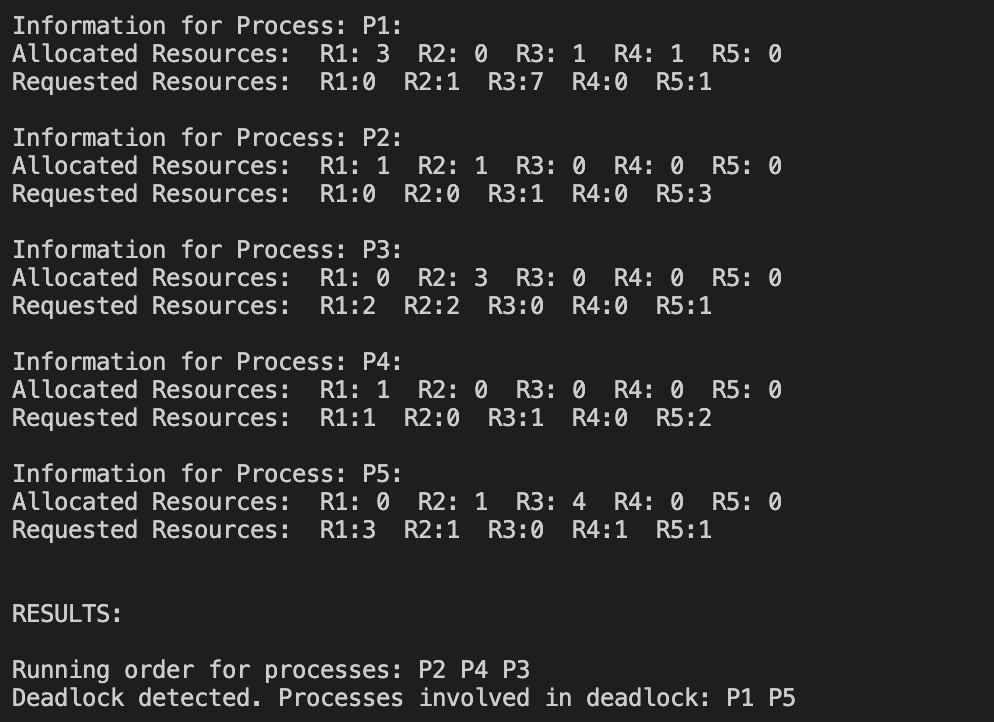
\includegraphics[width=0.75\textwidth]{output.png}
    \caption{Output for the given input files}
    \label{fig:output}
\end{figure}

\subsection{Discussion}
The Bankers' Algorithm is a helpful way to detect deadlocks before they happen, and it can ensure that a system remains concurrent and without any issues, and in this experiment, I was able to implement it in C language without problems and got the correct output as shown above.

\end{document}
